\chapter{Development}

\label{ch:Development}

\setlength{\parindent}{4em}
\setlength{\parskip}{1em}
\renewcommand{\baselinestretch}{1.5}

\section{Chamber for the experiment}

\begin{figure}[ht]
	\centering
	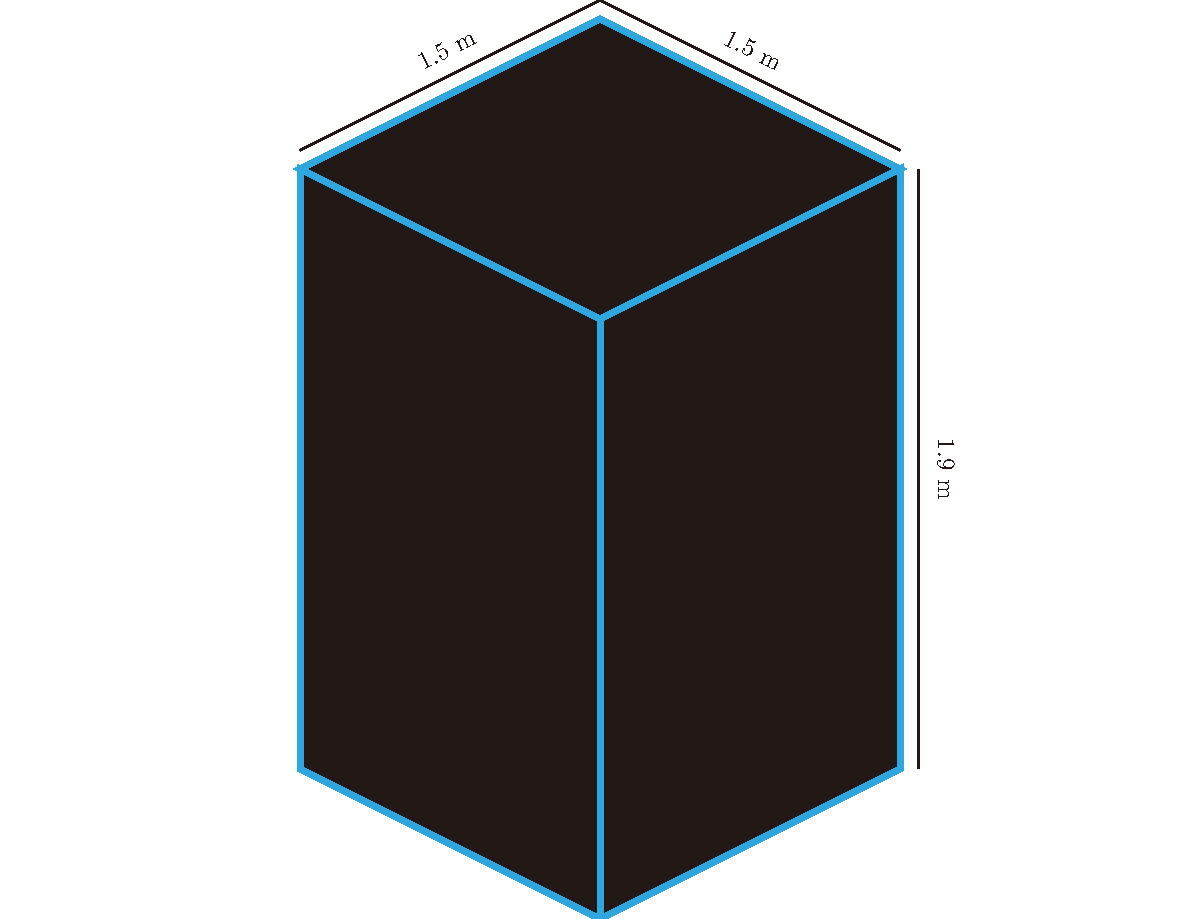
\includegraphics[width=0.8\textwidth]{chapter6/dark_wire.pdf}
	\caption{Experiment Chamber}
\end{figure}

\begin{figure}[ht]
	\centering
	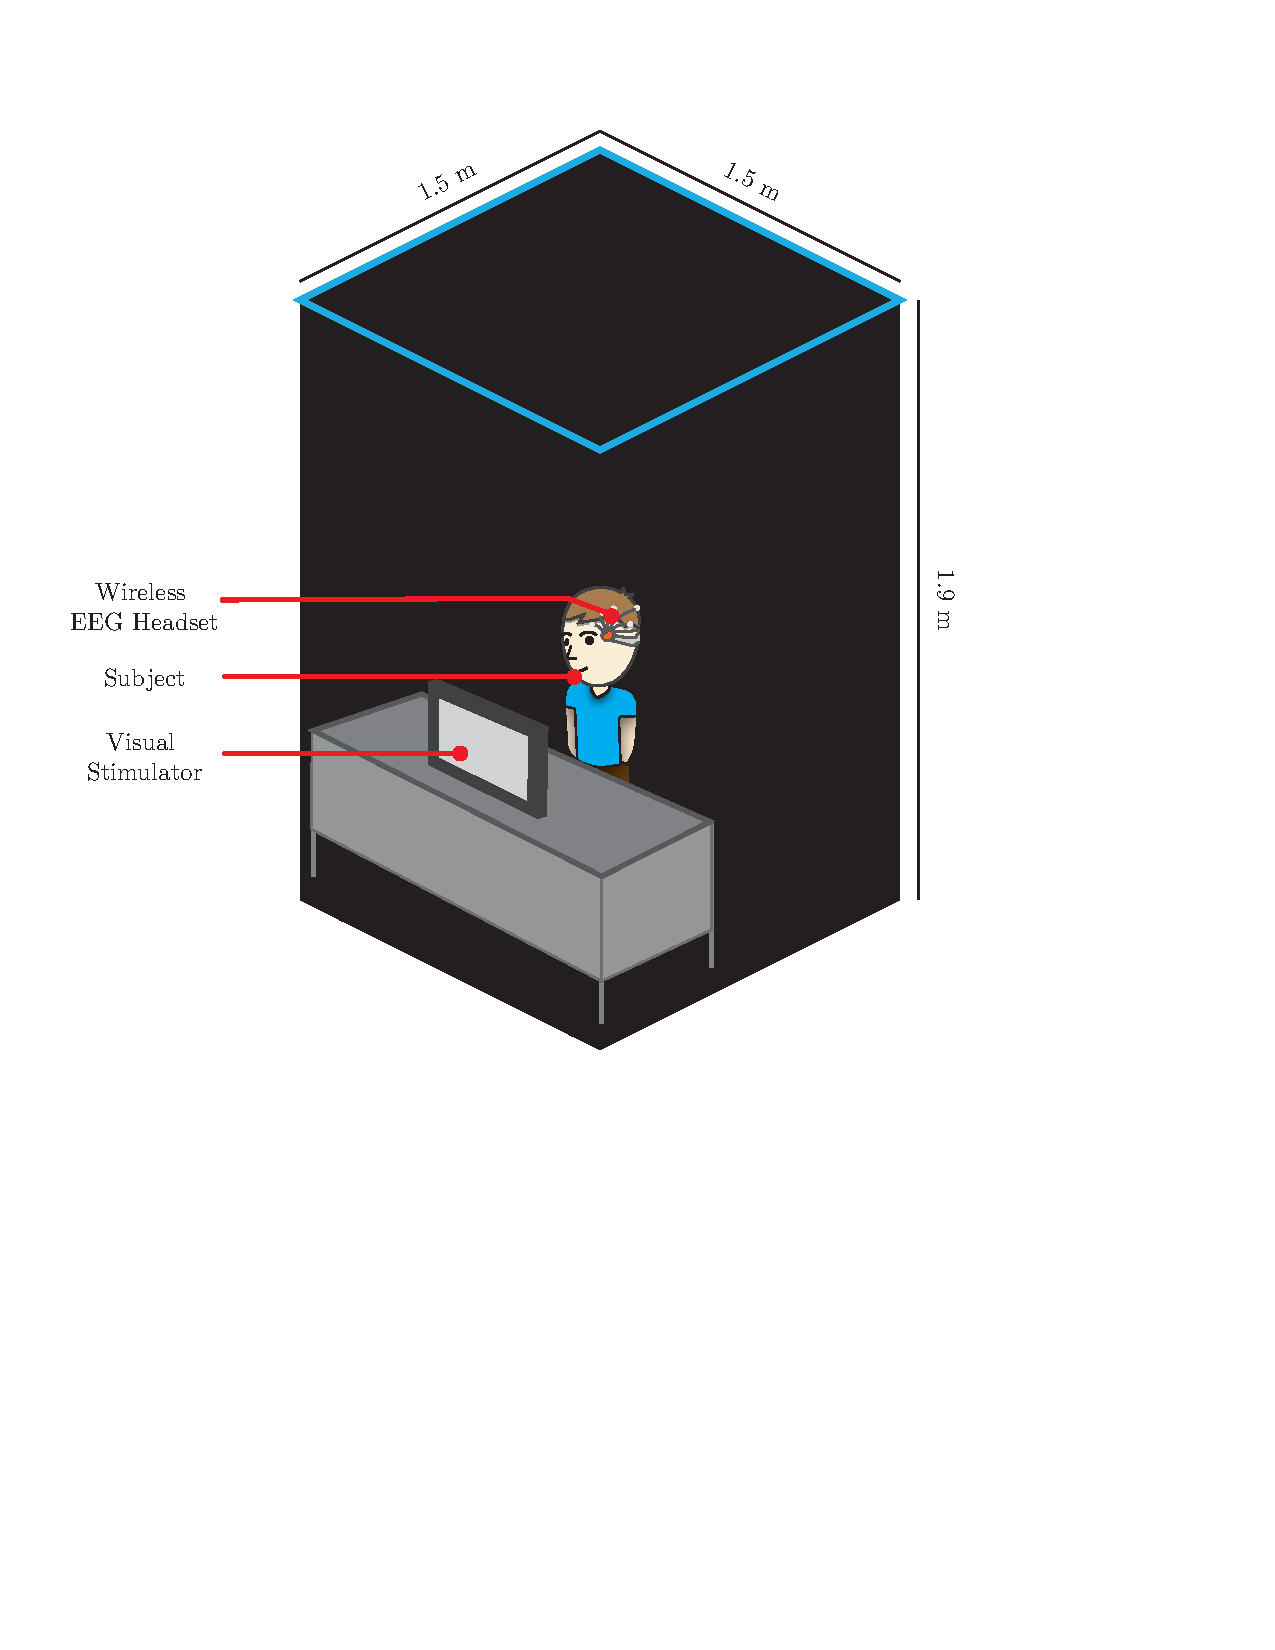
\includegraphics[width=0.8\textwidth]{chapter6/dark_wire_inside.pdf}
	\caption{Inside experiment Chamber}
\end{figure}

\begin{figure}[ht]
	\centering
	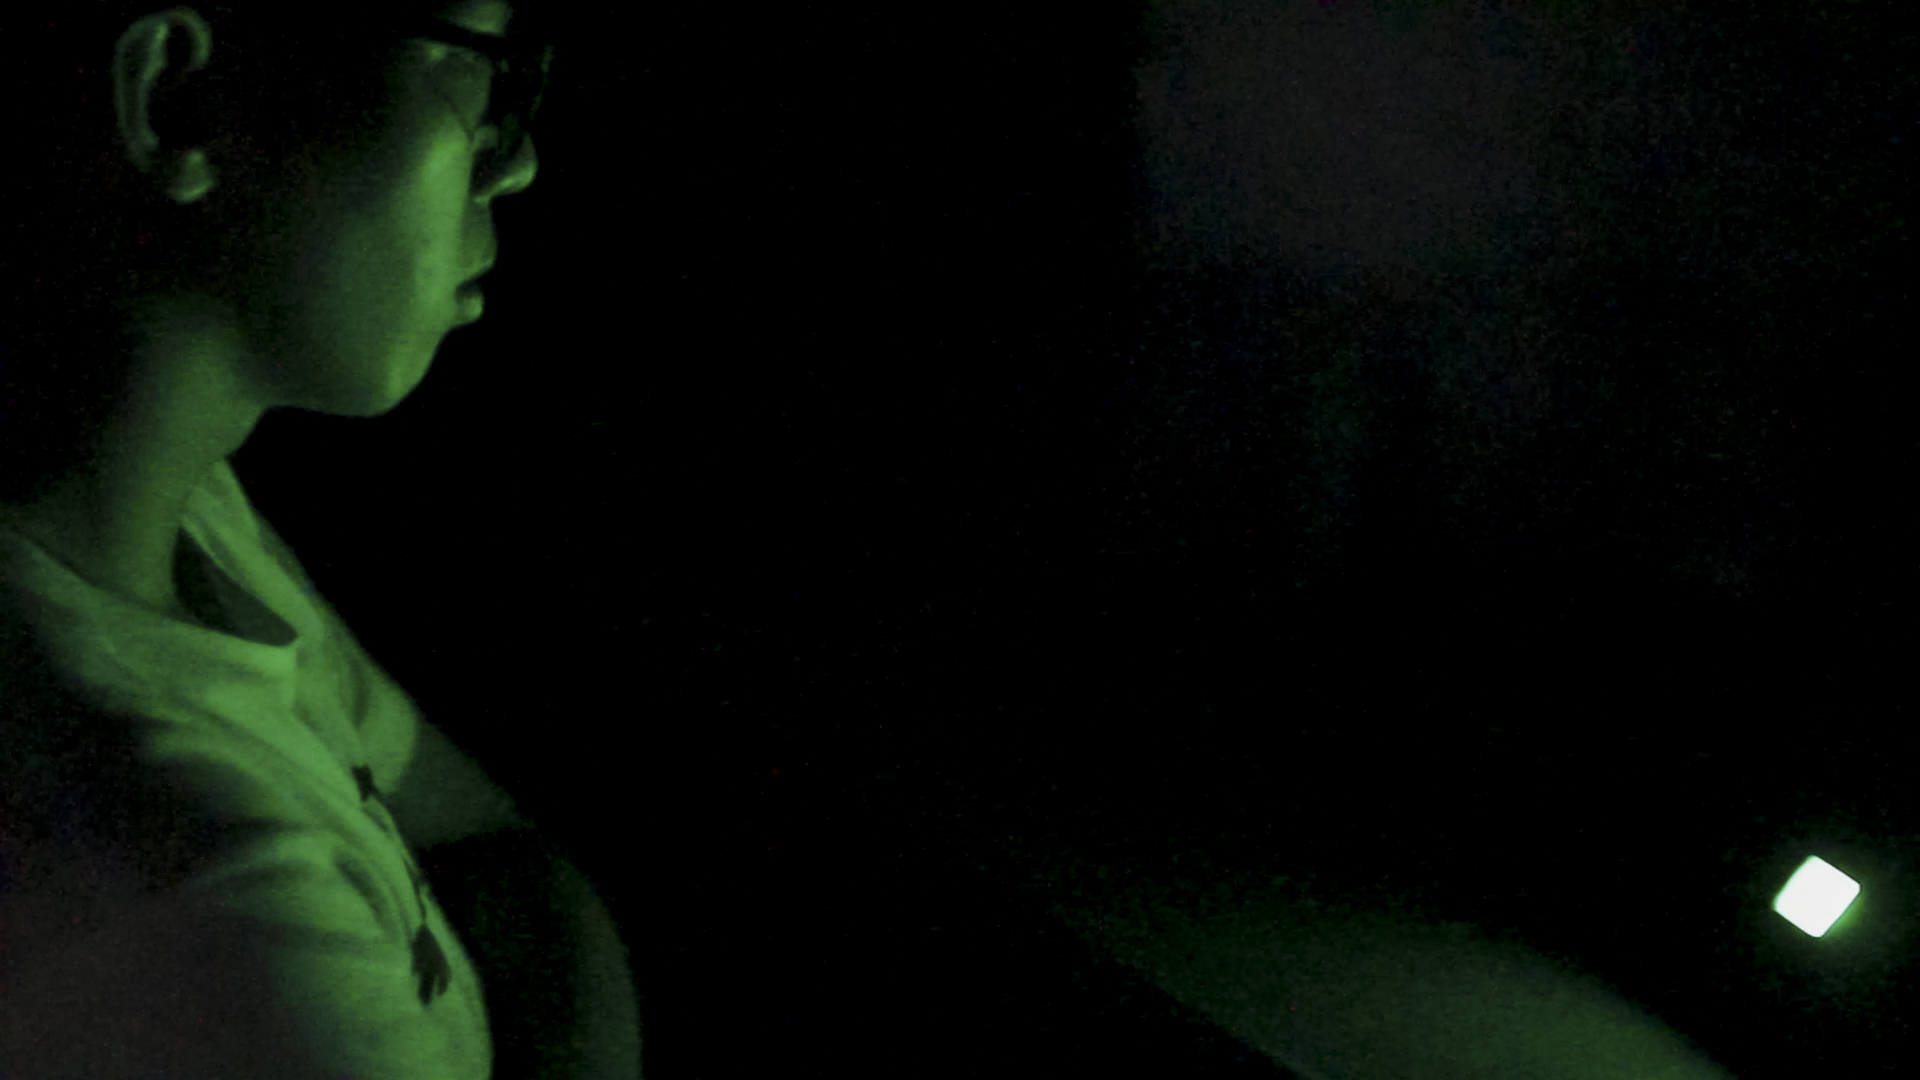
\includegraphics[width=0.8\textwidth]{chapter6/experi.jpg}
	\caption{While in experiment}
\end{figure}

\section{Visual stimulator}


\begin{figure}[ht]
	\centering
	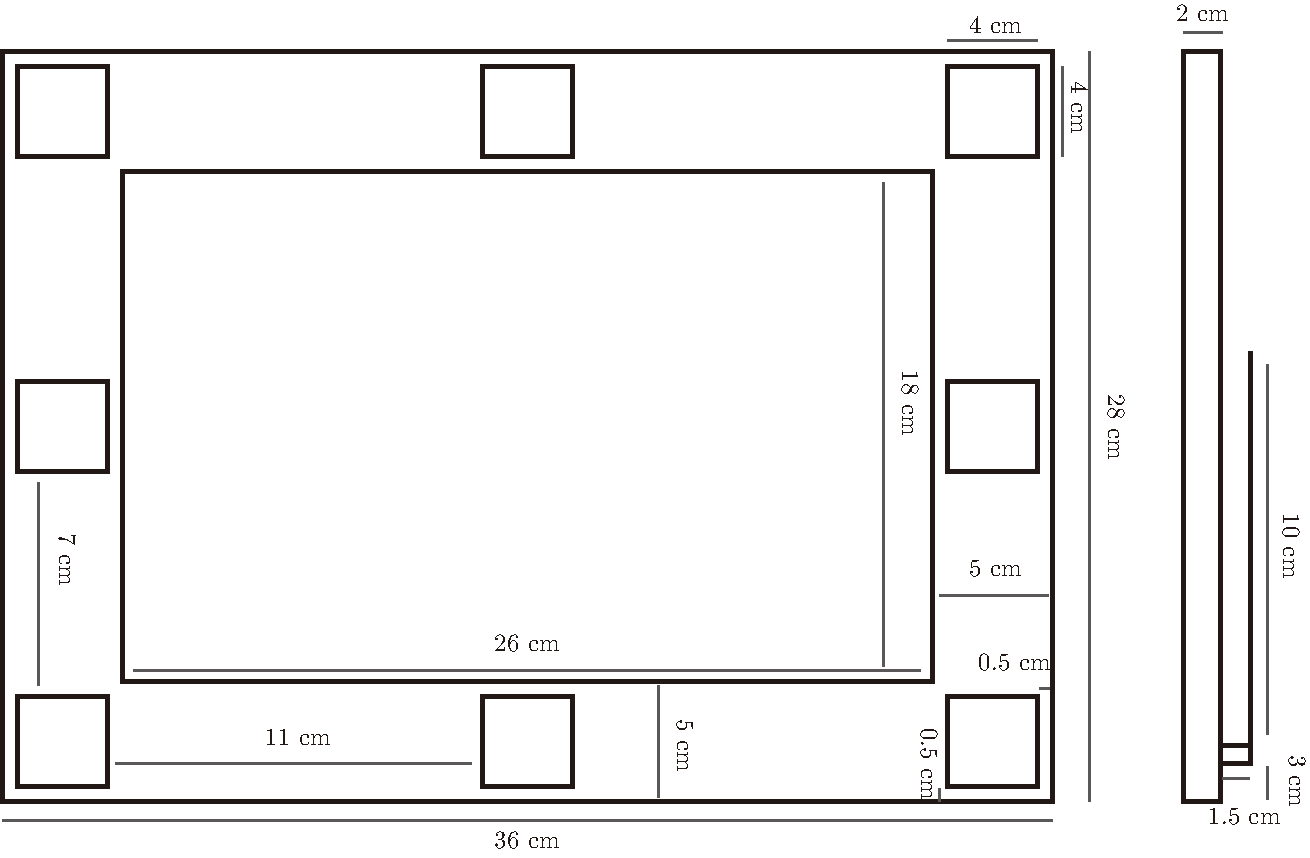
\includegraphics[width=0.8\textwidth]{chapter6/blueprint.pdf}
	\caption{Blueprint of Visual Stimulator}
\end{figure}

\begin{figure}[ht]
	\centering
	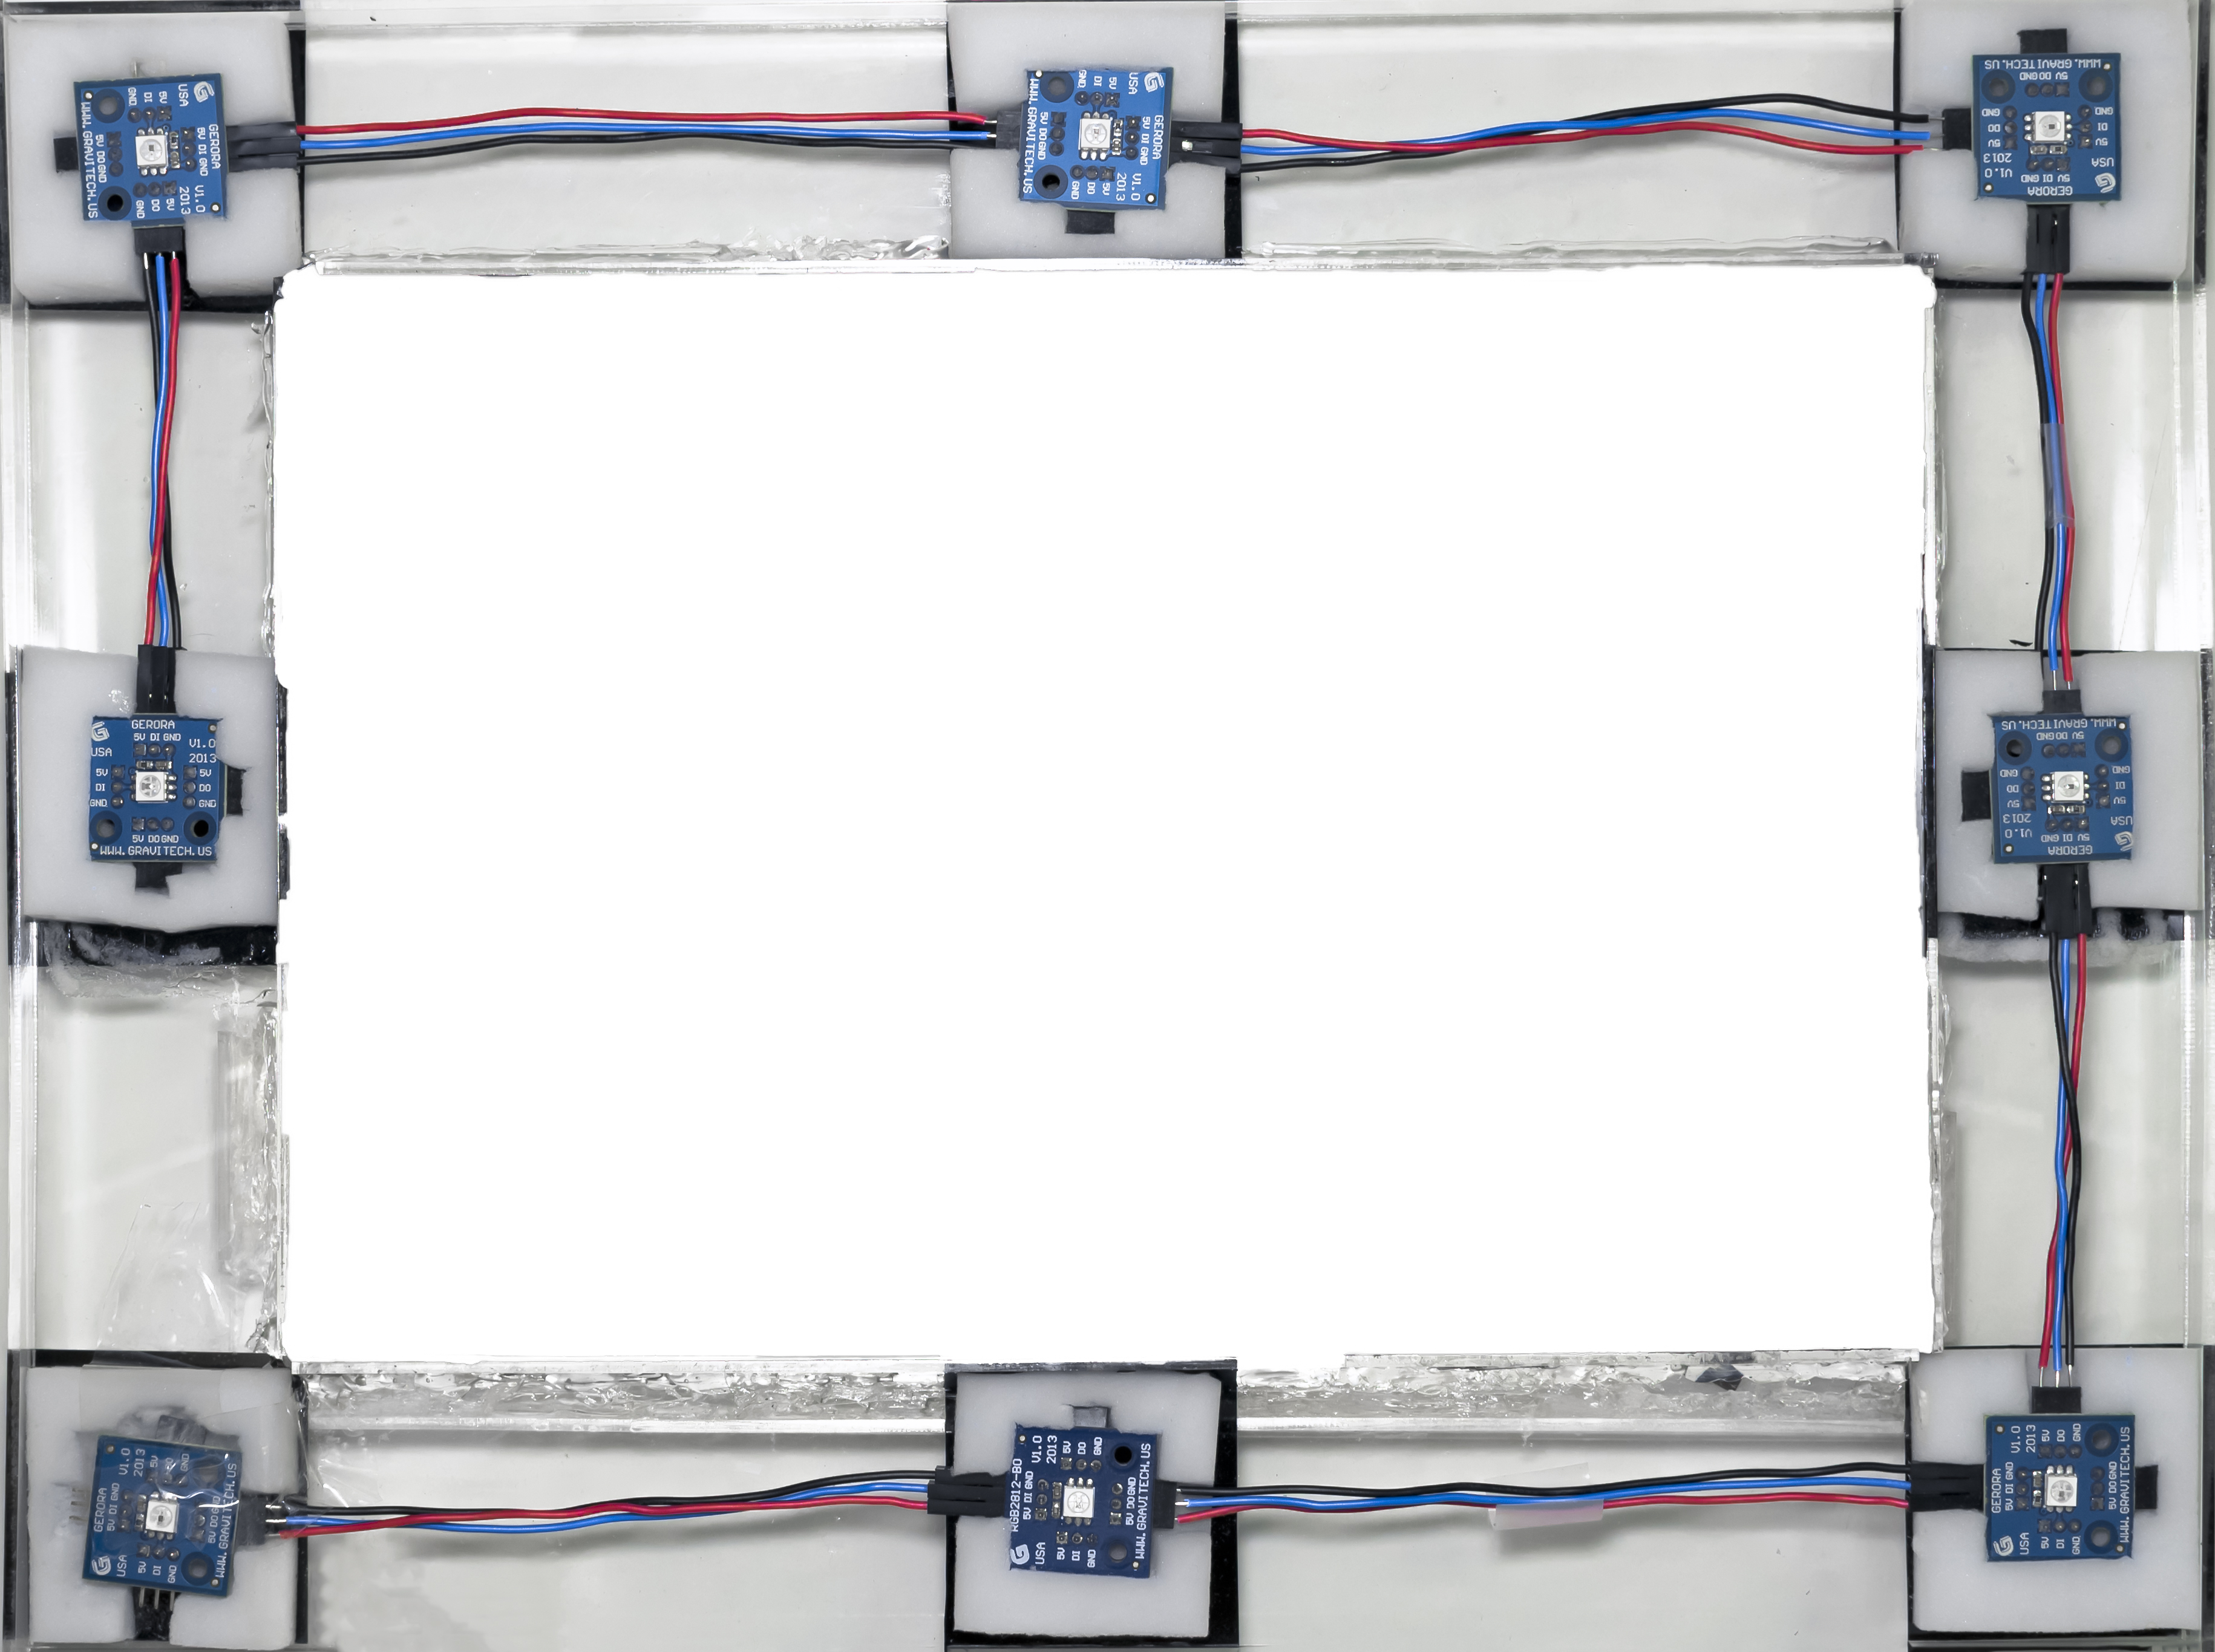
\includegraphics[width=0.8\textwidth]{chapter6/frame_LED.jpg}
	\caption{Visual Stimulator with LEDs wireing}
\end{figure}

\begin{figure}[ht]
	\centering
	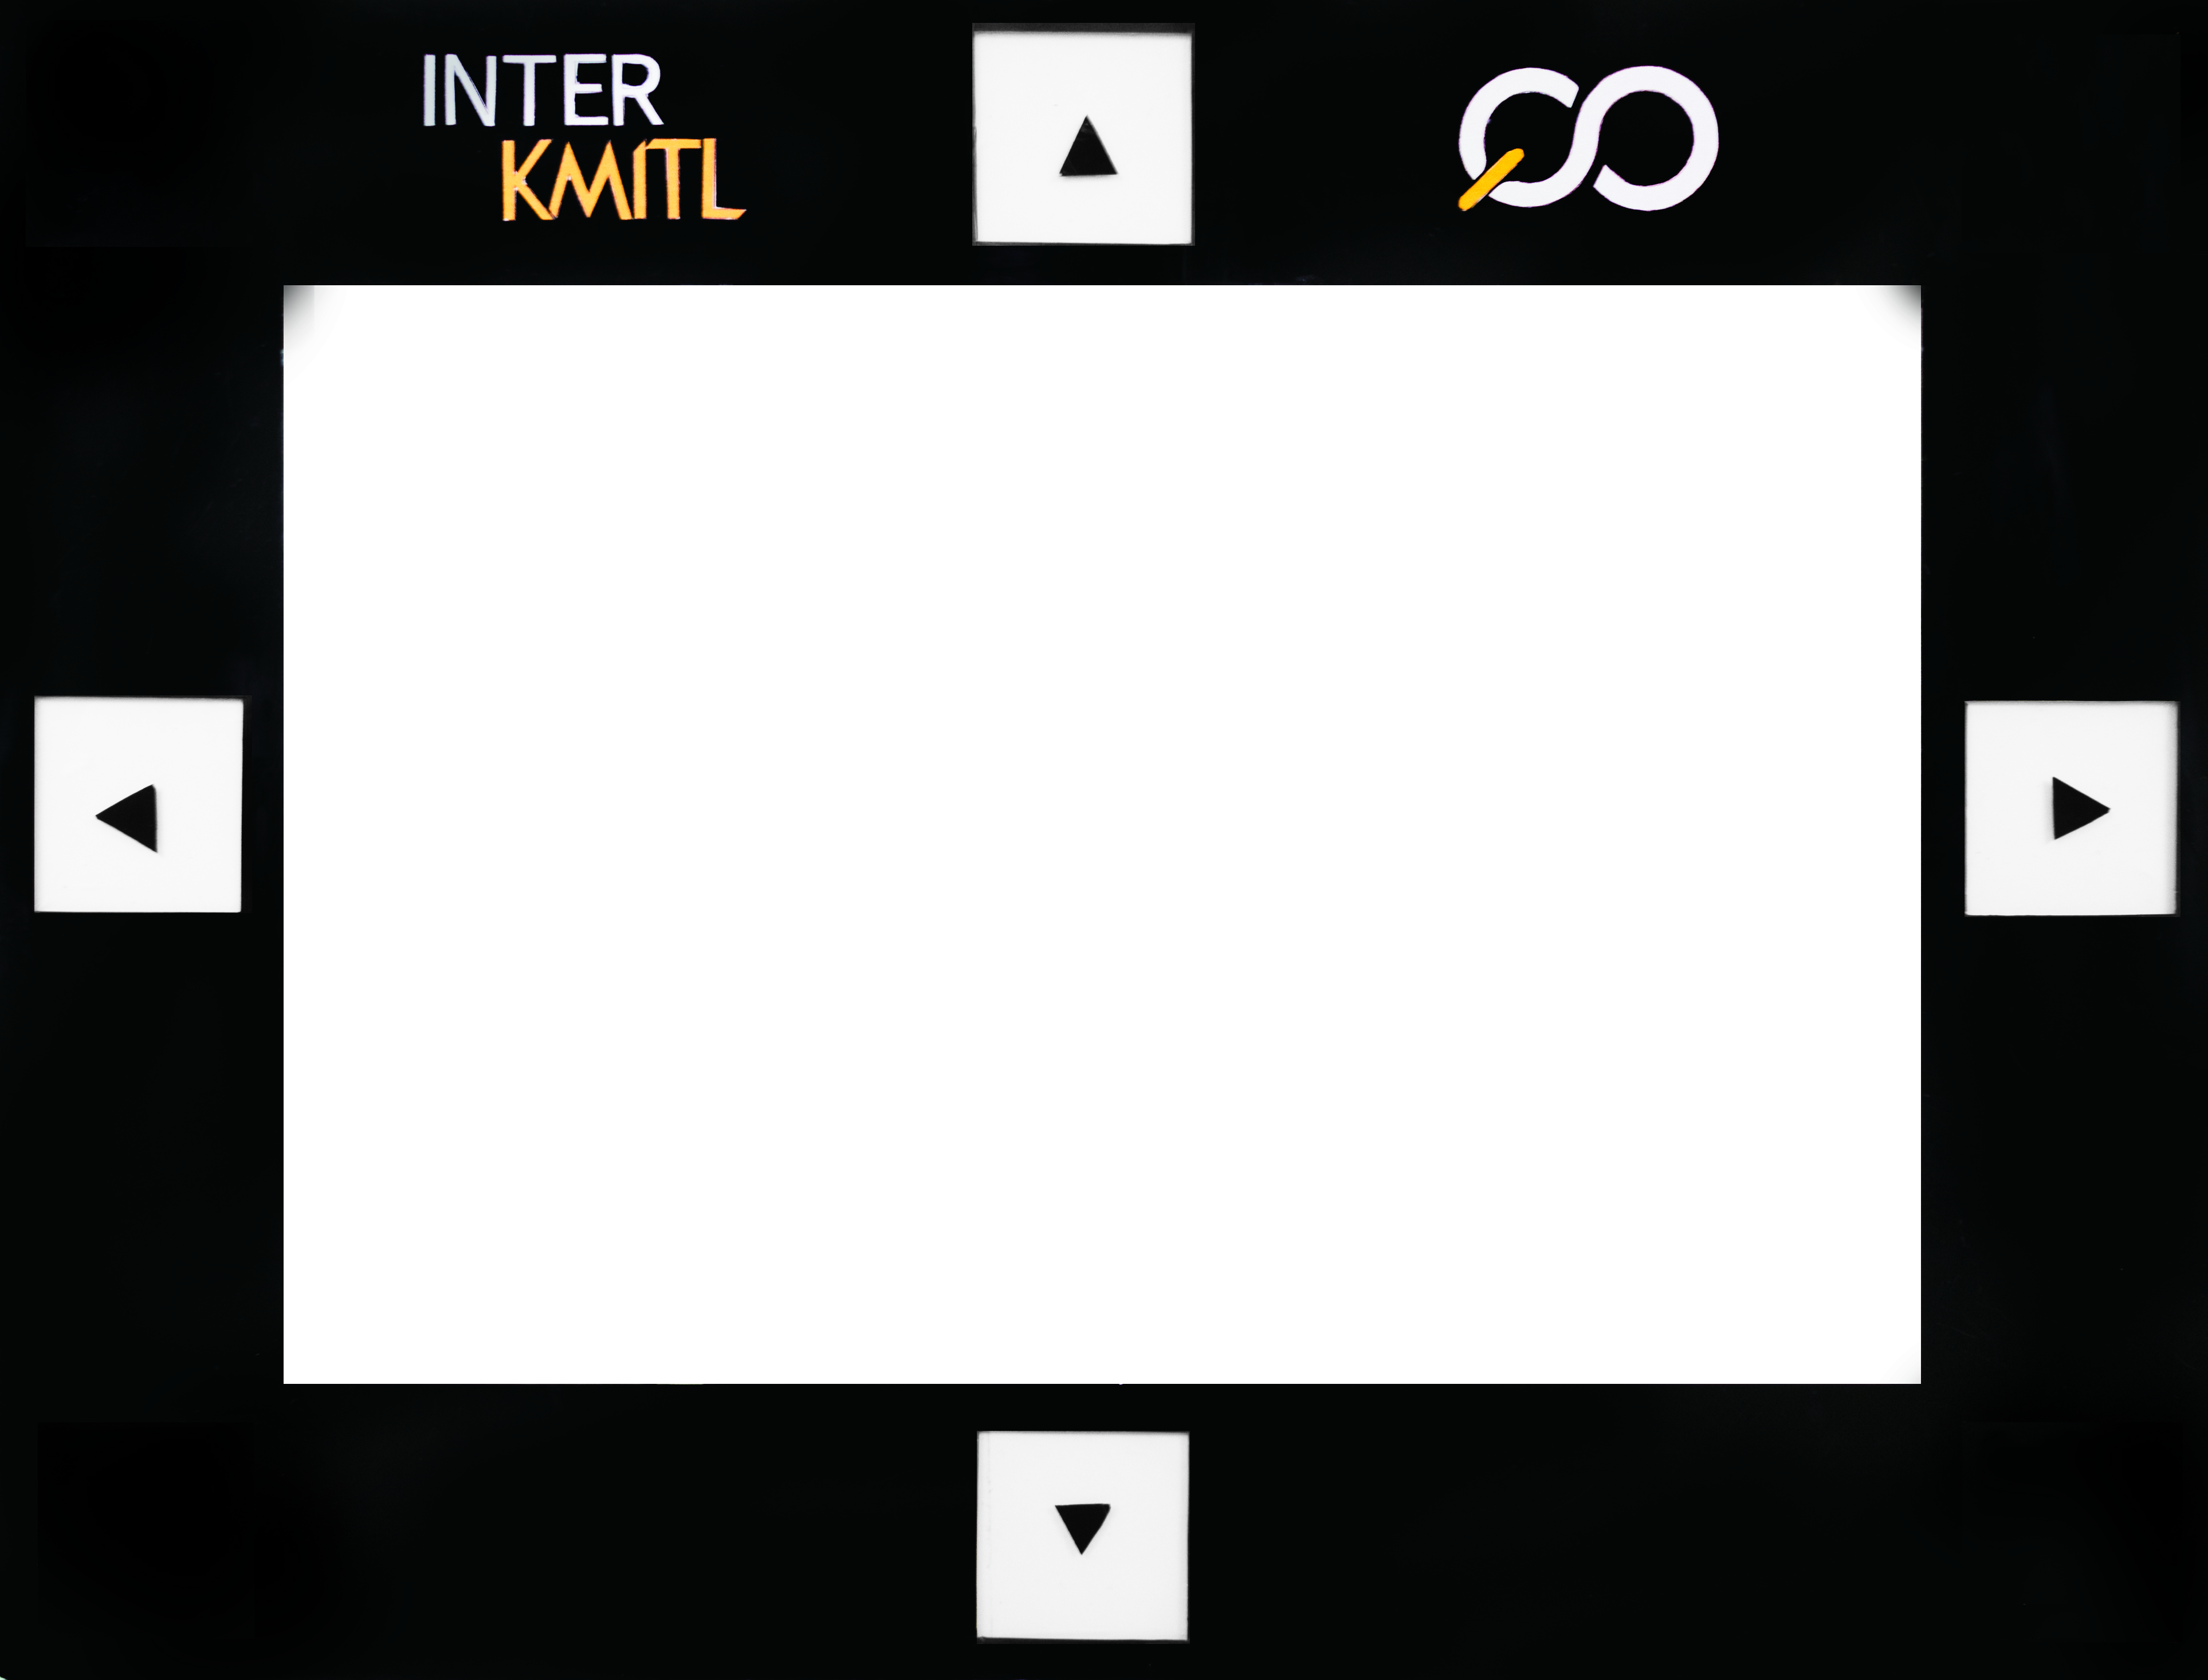
\includegraphics[width=0.8\textwidth]{chapter7/frame_4.jpg}
	\caption{Visual Stimulator with four targets used for ERPs}
\end{figure}

\begin{figure}[ht]
	\centering
	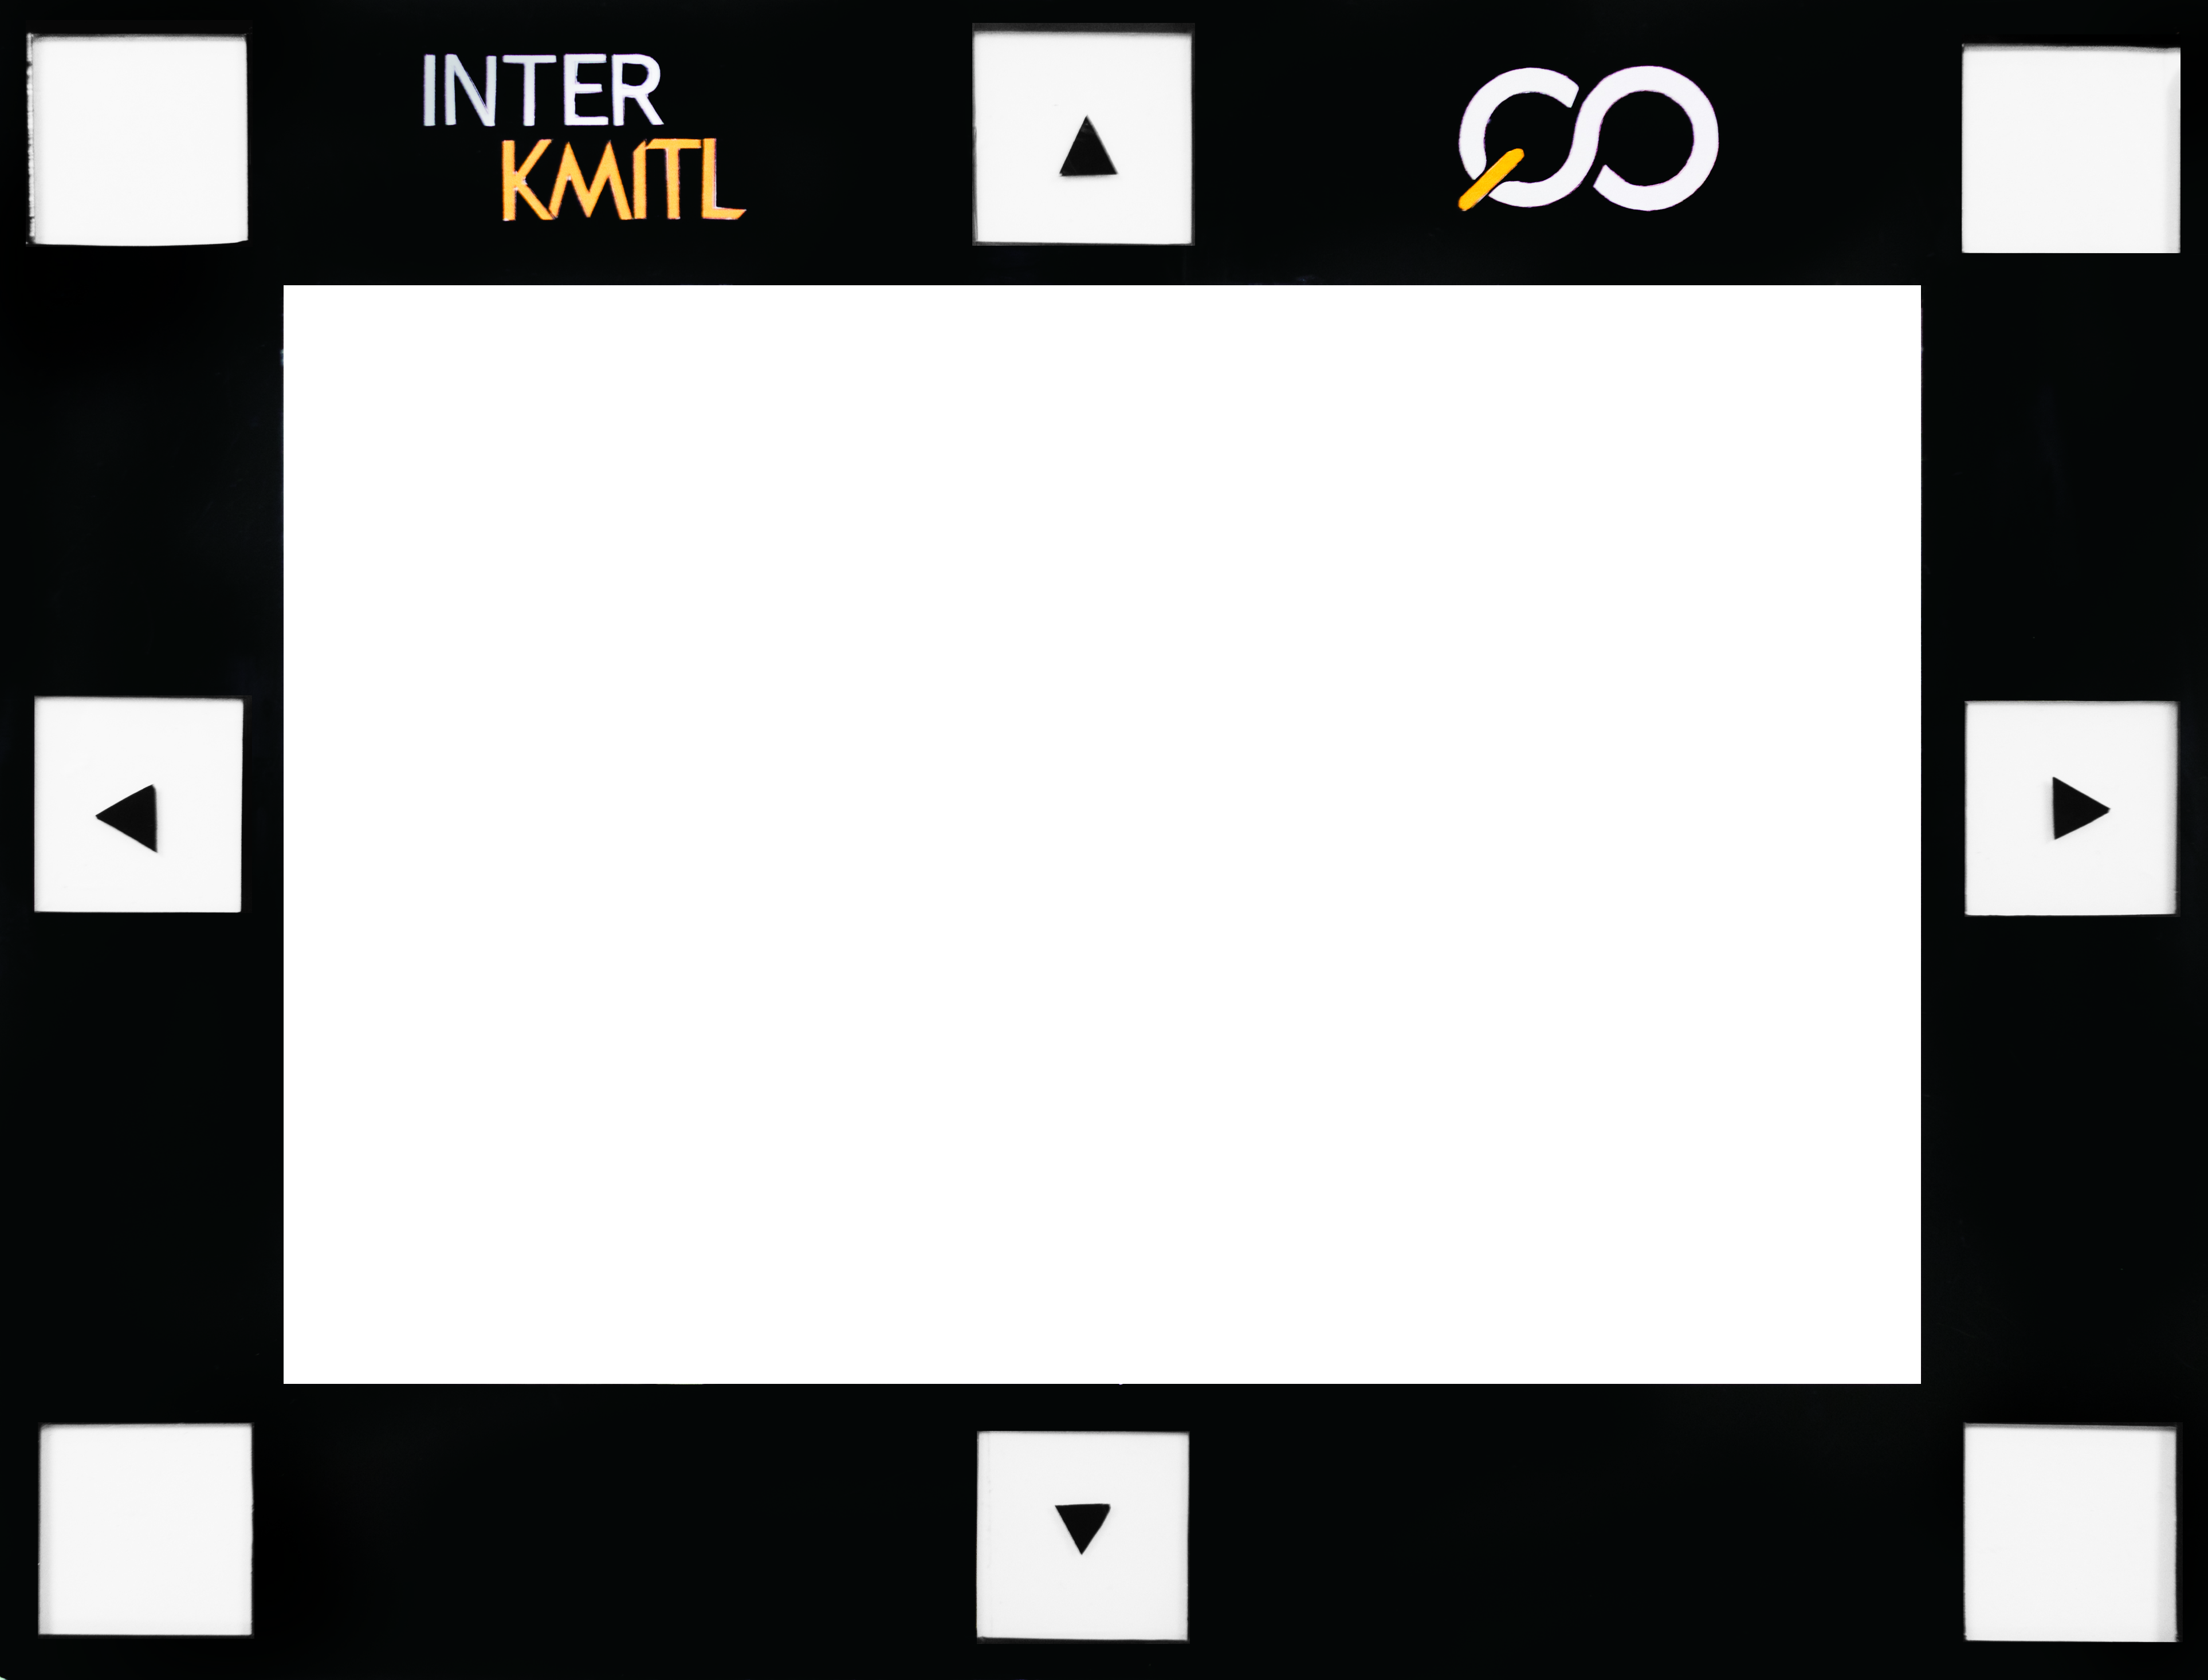
\includegraphics[width=0.8\textwidth]{chapter7/frame_8.jpg}
	\caption{Visual Stimulator with eight targets used for SSVEP}
\end{figure}

\section{Visual stimulator parameter}